\chapter{Hierarchical Routing}
\label{chap:hier-rtg}

This chapter describes the internals of hierarchical routing
implemented in \ns.
This chapter consists of two sections. In the first section we give an
overview of hierarchical routing. In the second section we walk through
the API's used for setting hierarchical routing and describe the
architecture, internals and code path for hier rtg in the process.

The functions and procedures described in this chapter can be found in
\nsf{tcl/lib/ns-hiernode.tcl, tcl/lib/ns-address.tcl,
  tcl/lib/ns-route.tcl and route.cc}. 

\section{Overview of Hierarchical Routing}
\label{sec:over-hier-rtg}

Hierarchical routing was mainly devised, among other things, to reduce
memory requirements of simulations over very large topologies. A
topology is broken down into several layers of hierarchy, thus
downsizing the routing table. The table size is reduced from 
{\em {$n^{2}$}}, for flat routing, to about {\em log n} for 
hierarchical routing. However some overhead costs results as 
number of hierarchy levels are increased. Optimum results were found for
3 levels of hierarchy and the current ns implementation supports upto a
maximum of 3 levels of hierarchical routing. 

To be able to use hierarchical routing for the simulations, we need to
define the hierarchy of the topology as well as provide the nodes with
hierarchical addressing. In flat routing, every node knows about every
other node in the topology, thus resulting in routing table size to the
order of 
$n^{2}$. For hierarchical routing, each node knows only about
those nodes in its level. For all other destinations outside its level
it forwards the packets to the border router of its level. Thus the
routing table size gets downsized to the order of about log n.

\section{Usage of Hierarchical routing}
\label{sec:usage-hier-rtg} 

Hierarchical routing requires some additional features and mechanisms
for the simualtion. For example, a new node object called {\em HierNode}
is been defined for hier rtg. Therefore the user must specify
hierarchical routing requirements before creating topology. This is done
as shown below: 

First, the address format (\label{chap:address} ) or the address space
used for node and port address, needs to be set in the hierarchical
mode. It may be done in one of the two ways:

\begin{program}
  set ns [new Simulator]
  \$ns set-address-format hierarchical
\end{program} 

This sets the node address space to a 3 level hierarchy assigning 8 bits
in each level.

or,
\begin{program}
  \$ns set-address-format hierarchical <n hierarchy levels> <\# bits in
  level 1> ...<\# bits in nth level>
\end{program} 

which creates a node address space for n levels of hierarchy assigning
bits as specified for every level.

This other than creating a hierarchical address space also sets a flag
called {\em EnableHierRt\_} and sets the Simulator class variable
node\_factory\_ to HierNode.  
Therefore when nodes are created by calling Simulator method ``node'' as
in :

\$ns node 0.0.1,
a HierNode is created with an address of 0.0.1;

Class AddrParams is used to store the topology hierarchy like number
of levels of hierarchy, number of areas in each level like number of
domains, number of clusters and number of nodes in each cluster.

The API for supplying these information to AddrParams is shown below:

\begin{program}
AddrParams set domain_num_ 2
lappend cluster_num 2 2
AddrParams set cluster_num_ \$cluster_num
lappend eilastlevel 2 3 2 3
AddrParams set nodes_num_ \$eilastlevel
\end{program}

This defines a topology with 2 domains, say D1 and D2 with 2 clusters
each (C11 \& C12 in D1 and C21 \& C22 in D2). Then number of nodes in
each of these 4 clusters is specified as 2,3,2 and 3 respectively.

The default values used by AddrParams provide a topology with a single
domain with 4 clusters, with each cluster consisting of 5 nodes.

Appropriate mask and shift values are generated by AddrParams for the
hierarchical node address space.

Each HierNode at the time of its creation calls the method
`mk-default-classifier '' to setup n numbers of address
classifiers for n levels of hierarchy defined in the topology.

\begin{program}
  HierNode instproc mk-default-classifier {} {
    \$self instvar np_ id_ classifiers_ agents_ dmux_ neighbor_ address_ 
    # puts "id=\$id_"
    set levels [AddrParams set hlevel_]
    for {set n 1} {\$n <= \$levels} {incr n} {
      set classifiers_(\$n) [new Classifier/Addr]
      \$classifiers_(\$n) set mask_ [AddrParams set NodeMask_(\$n)]
      \$classifiers_(\$n) set shift_ [AddrParams set NodeShift_(\$n)]
      }
    }
\end{program}

At the time of route computation, a call is made to add-route.
add-route populates classifiers as shown in the otcl method below:

\begin{program}
Node instproc add-route { dst target } {
 	\$self instvar rtnotif_
	# Notify every module that is interested about this 
	# route installation
	
	if {\$rtnotif_ != ""} {
		\$rtnotif_ add-route \$dst \$target
	}
	\$self incr-rtgtable-size
}
\end{program}

For an example of 3 level of hierarchy, the level 1 classifier demuxes
for domains, level 2 for all clusters inside the node's domain and
finally classifier 3 demuxes for all nodes in the particular cluster
that the node itself resides. For such a topology, a HierNode with
address of 0.1.2 looks like the figure below:
\begin{figure}[tb]
\centerline{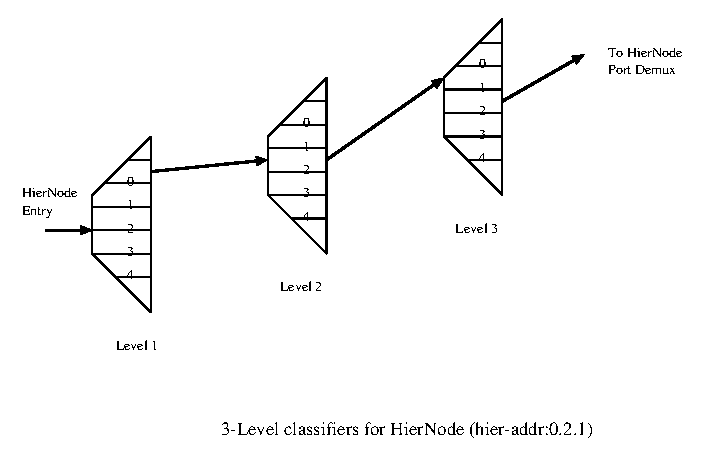
\includegraphics{hier-classifier}}
\caption{Hierarchical classifiers}
\label{fig:hier-classifier}
\end{figure}

Thus the size of the routing tables are considerably reduced from 
$n^{2}$ as seen for flat routing where each node had to store the
  next\_hop info of all other nodes in the topology. Instead, for
  hierarchical routing, a given node needs to know about its neighbours
  in its own cluster, about the all clusters in its domain and about all
  the domains. This saves on memory consumption as well as run-time for
  the simulations using several thousands of nodes in their topology.


\section{Creating large Hierarchical topologies}
\label{large-hier-topo}
The previous section describes methods to create hierarchical topologies
by hand. However, there is a script available in ns that converts
Georgia-tech's SGB-graphs into ns compatible hierarchical topologies.
Please refer to {\em http://www-mash.CS.Berkeley.EDU/ns/ns-topogen.html}
for downloading as well as instructions on using the hierarchical
converter package. 

See hier-rtg-10.tcl and hier-rtg-100.tcl in \nsf{tcl/ex} for example
scripts of hier routing on small and large topologies
respectively. 


\section{Hierarchical Routing with SessionSim}
\label{sec:hier-rtg-with-sessionsim}

Hierarchical routing may be used in conjunction with Session simulations
(see Chapter ~\ref{chap:session}). Session-level simulations which are used
for running multicast simulations over very large topologies, gains
additionally in terms of memory savings if used with hierarchical
routing. See simulation script \nsf{tcl/ex/newmcast/session-hier.tcl}
for an example of sessionsim over hier rtg.


\section{Commands at a glance}

Following is a list of hierarchical routing/addressing related commands
used in simulation scripts:
\begin{flushleft}
\code{$ns_ set-address-format hierarchical}\\
This command was used to setup hierarchical addressing in \ns. However with
the recent changes in node APIs, this command has been replaced by\\
\code{ns_ node-config -addressType hierarchical}\\
This creates a default topology of 3 levels of hierarchy, assigning 8 bits
to each level.


\code{$ns_ set-address-format hierarchical <nlevels> <#bits in level1>....<#bits in level n>}\\
This command creates a hierarchy of <nlevels> and assigns the bits in each level
as specified in the arguments.


\begin{program}
AddrParams set domain_num_ <n_domains>
AddrParams set cluster_num_ <n_clusters>
AddrParams set nodes_num_ <n_nodes>
\end{program}
The above APIs are used to specify the hierarchical topology, i.e the number of
domains, clusters and nodes present in the topology. Default values used by
AddrParams (i.e if nothing is specified) provide a topology with a single
domain with 4 clusters, with each cluster consisting of 5 nodes.


Internal procedures:\\

\code{$Node add-route <dst> <target>}\\
This procedure is used to add next-hop entries of a destination <dst> for a given <target>. 


\code{$hiernode_ split-addrstr <str>}\\
This splits up a hierarchical adrress string  (say a.b.c) into a list of
the addresses at each level (i.e, a,b and c).

\end{flushleft}

\endinput
